%-------- Document Class  ------------------------------------------------------------------------------------------------------------------------------------------------
\documentclass[a4paper,10pt,smallheadings]{scrartcl}
\usepackage[margin=1cm
%,showframe% <- only to show the page layout
]{geometry}
\usepackage[utf8]{inputenc}

%-------- Multi-file  ---------------------------------------------------------------------------------------------------------------------------------------------------------
\usepackage{subfiles}

%-------- Preambolo  --------------------------------------------------------------------------------------------------------------------------------------------------
%Per le Figure
\usepackage[english]{babel}
\usepackage{graphicx}

%simboli matematici strani quali unione disgiunta
\usepackage{amssymb}

%Scrivere Sotto i simboli
\usepackage{amsmath}

%Diagrammi Commutativi
\usepackage{tikz}
\usetikzlibrary{matrix}

%Il simbolo di Identità
\usepackage{dsfont}

%Per riflettere i simboli...
\usepackage{graphicx}


%link iNTERNET
\usepackage{hyperref}

%Enumerate with letters
\usepackage{enumerate}

%Slash over letter
\usepackage{cancel}

%Usare bibiliografia bibtex
%\bibliographystyle{plain}

%Danger sign
\usepackage{fourier}

%:=
\usepackage{mathtools}

%http://tex.stackexchange.com/questions/8625/force-figure-placement-in-text
\usepackage{caption}


%subsection numbering
 \setcounter{tocdepth}{3} % if you want all the levels in your table of contents

%Common symbols
%Common math symbols
	%Number fields
		\newcommand{\Real}{\mathbb{R}}
		\newcommand{\Natural}{\mathbb{N}}
		\newcommand{\Relative}{\mathbb{Z}}
		\newcommand{\Rational}{\mathbb{Q}}
		\newcommand{\Complex}{\mathbb{C}}
	
%equality lingo
	%must be equal
		\newcommand{\mbeq}{\overset{!}{=}} 

% function
	%Domain
		\newcommand{\dom}{\mathrm{dom}}
	%Range
		\newcommand{\ran}{\mathrm{ran}}
	

% Set Theory
	% Power set (insieme delle parti
		\newcommand{\PowerSet}{\mathcal{P}}

%Differential Geometry
	% Atlas
		\newcommand{\Atlas}{\mathcal{A}}
	%support
		\newcommand{\supp}{\textrm{supp}}

	
	
%Category Theory
	%Mor set http://ncatlab.org/nlab/show/morphism
%		\newcommand{\hom}{\textrm{hom}}

%Geometric Lagrangian Mechanics
	% Kinematic Configurations
		\newcommand{\Conf}{\mathtt{C}}
	%Solutions Space
		\newcommand{\Sol}{\mathtt{Sol}}
	%Lagrangian class
		\newcommand{\Lag}{\mathsf{Lag}}
	%Lagrangiana
		\newcommand{\Lagrangian}{\mathcal{L}}
	%Data
		\newcommand{\Data}{\mathsf{Data}}
	%unique solution map
		\newcommand{\SolMap}{\mathbf{s}}
	%Classical Observables
		\newcommand{\Obs}{\mathcal{E}}	
	%Phase Space
		\newcommand{\Phase}{\mathcal{M}}	

		\
		
%Peierls (per non sbagliare più)
		\newcommand{\Pei}{Peierls}

%Accented Letters
\usepackage[utf8]{inputenc}

%Temporaneo, Aggiunta della mia classe teorem... Deve diventare un pacchetto!
\input{../Latex-Theorem/TheoremTemplateToninus.tex}
%Common math symbols
	%Number fields
		\newcommand{\Real}{\mathbb{R}}
		\newcommand{\Natural}{\mathbb{N}}
		\newcommand{\Relative}{\mathbb{Z}}
		\newcommand{\Rational}{\mathbb{Q}}
		\newcommand{\Complex}{\mathbb{C}}
	
%equality lingo
	%must be equal
		\newcommand{\mbeq}{\overset{!}{=}} 

% function
	%Domain
		\newcommand{\dom}{\mathrm{dom}}
	%Range
		\newcommand{\ran}{\mathrm{ran}}
	

% Set Theory
	% Power set (insieme delle parti
		\newcommand{\PowerSet}{\mathcal{P}}

%Differential Geometry
	% Atlas
		\newcommand{\Atlas}{\mathcal{A}}
	%support
		\newcommand{\supp}{\textrm{supp}}

	
	
%Category Theory
	%Mor set http://ncatlab.org/nlab/show/morphism
%		\newcommand{\hom}{\textrm{hom}}

%Geometric Lagrangian Mechanics
	% Kinematic Configurations
		\newcommand{\Conf}{\mathtt{C}}
	%Solutions Space
		\newcommand{\Sol}{\mathtt{Sol}}
	%Lagrangian class
		\newcommand{\Lag}{\mathsf{Lag}}
	%Lagrangiana
		\newcommand{\Lagrangian}{\mathcal{L}}
	%Data
		\newcommand{\Data}{\mathsf{Data}}
	%unique solution map
		\newcommand{\SolMap}{\mathbf{s}}
	%Classical Observables
		\newcommand{\Obs}{\mathcal{E}}	
	%Phase Space
		\newcommand{\Phase}{\mathcal{M}}	

		\
		
%Peierls (per non sbagliare più)
		\newcommand{\Pei}{Peierls}	%Common symbols
\usepackage{glossaries}

\makenoidxglossaries

%How to:
%affinchè la voce venga printata nella lista va prima chiamata nel testo come e.g. \gls{Bundle}
%ricordarsi di chiamarlo almeno una volta così, dopo usare il command per evitare il ripetuto hyperref
% anche se si potrebbe evitare visto che il quadratino del link non dovrebbe apparire in stampa

%Advanced Differential Geometry
\newglossaryentry{Bundle}%
{%
	name={\ensuremath{E = (E,\pi , M;Q)}},
	description={ Fiber Bundles $\pi: E\rightarrow M$ with typical fiber $Q$},
    sort={B}
}

\newglossaryentry{Sections}%
{%
	name={\ensuremath{\Gamma^\infty(E)}},
	description={ Smooth sections on the bundle $E$.},
    sort={S}
}


%Geometric Lagrangian Mechanics
	% Kinematic Configurations
	\newglossaryentry{Conf}%
	{%
		name={\ensuremath{\Conf}},
		description={ Kinematic Configurations set}
	}

	%Solutions Space
	\newglossaryentry{Sol}%
	{%
		name={\ensuremath{\Sol}},
		description={ Dynamic Configurations set}
	}

		
	%Lagrangian class
		\newglossaryentry{Lag}%
	{%
		name={\ensuremath{\Lag}},
		description={ Set of Lagrangian densities.}
	}
		
	%Lagrangiana
	\newglossaryentry{Lagrangian}%
	{%
		name={\ensuremath{\Lagrangian}},
		description={ Lagriangian density of the system.}
	}
		
	%Data
	\newglossaryentry{Data}%
	{%
		name={\ensuremath{\Data}},
		description={ Inital Data set.}
	}
		
	%unique solution map
	\newglossaryentry{SolMap}%
	{%
		name={\ensuremath{\SolMap}},
		description={ Map that map a fixed initial data to the unique solution.}
	}
		
	%Classical Observables
	\newglossaryentry{Obs}%
	{%
		name={\ensuremath{\Obs}},
		description={ Set of all classical observables.}
	}

	%Phase Space
	%Classical Observables
	\newglossaryentry{Phase}%
	{%
		name={\ensuremath{\Phase}},
		description={ Phase space.}
	}



\hyphenation{gua-ran-te-ed}
\hyphenation{Ha-da-mard}
\hyphenation{Rieman-nian}
\pagestyle{empty}

%Temporaneo, Aggiunta della mia classe teorem... Deve diventare un pacchetto!
\input{../../Latex-Theorem/TheoremTemplateToninus.tex}

%---------------------------------------------------------------------------------------------------------------------------------------------------------------------
\title{Demystification of Peierels Brackets construction}
\author{Antonio Michele Miti}
\date{\vspace{-5ex}} % workaround to omit the Date !

%\/\/\/\/\/\/\/\/\/\/\/\/\/\/\/\/\/\/\/\/\/\/\/\/\/\/\/\/\/\/\/\/\/\/\/\/\/\/\/\/\/\/\/\/\/\/\/\/\/\/\/\/\/\/\/\/\/\/\/\/\/\/\/\/\/\/\/\/\/
\begin{document} %\/\/\/\/\/\/\/\/\/\/\/\/\/\/\/\/\/\/\/\/\/\/\/\/\/\/\/\/\/\/\/\/\/\/\/\/\/\/\/\/\/\/\/\/\/\/\/\/\/\/\/\/\/\/\/\/\/\/\/

\section{Fiber Bundles}
\begin{definition}[Fiber Bundle]\label{Def:SmoothBundle}
				We call a \emph{Smooth (Fiber) Bundle}  a quadruple $E = (E,M,Q,\pi)$ where:
				\begin{itemize}
					\item[-] $E,M,Q$ :  smooth manifolds called respectively \emph{Total Space}, \emph{Base Space}, \emph{Typical Fiber}.
					\item[-] $\pi : E \rightarrow M $ smooth, everywhere defined, surjective function (called \emph{Bundle Projection})
				\end{itemize}
				Such that $\forall x \in M \quad \exists$ a \emph{local trivialization}) $(U, \chi)$.
				
	\end{definition}
	
	\begin{definition}[Local Trivialization of the Fiber Bundle $E$]				
		A Pair $(U, \chi)$ where:
					\begin{compactitemize}
						\item $U$ : neighbourhood of $x \in M$
						\item $\chi$ :$\pi^{-1}(U) \rightarrow U \times Q$ : diffeomorphism
							%DaRivedere
 							\footnote{surjectivity $\Rightarrow$ $\pi^{-1}(U) \neq \emptyset$.}
 							\footnote{cartesian product of topological space is a topological space with the direct product topology.}
					\end{compactitemize}
				such that the natural projection $p_1 : U \times F \rightarrow U$ satisfies the following equation: $$p_1 \cdot \chi = \pi \vert_{\pi^{-1}(p)}$$
					\textit{i.e.}: the following graph commutes:
					\vspace{-2mm}
					\begin{center}
					\begin{tikzpicture}
						 \matrix (m) [matrix of math nodes,row sep=3em,column sep=4em,minimum width=2em] {
     						\pi^{-1}(U) & U \times Q \\
     						U &  \\};
 						 \path[-stealth]
 							(m-1-1) edge node [left] {$\pi$} (m-2-1)
            				edge [right] node [above] {$\chi$} (m-1-2)
    						(m-1-2) edge [right] node [below] {$p_{1}$} (m-2-1);;
					\end{tikzpicture}
					\end{center}
			\end{definition}

			\begin{figure}[h!]
				\centering
  				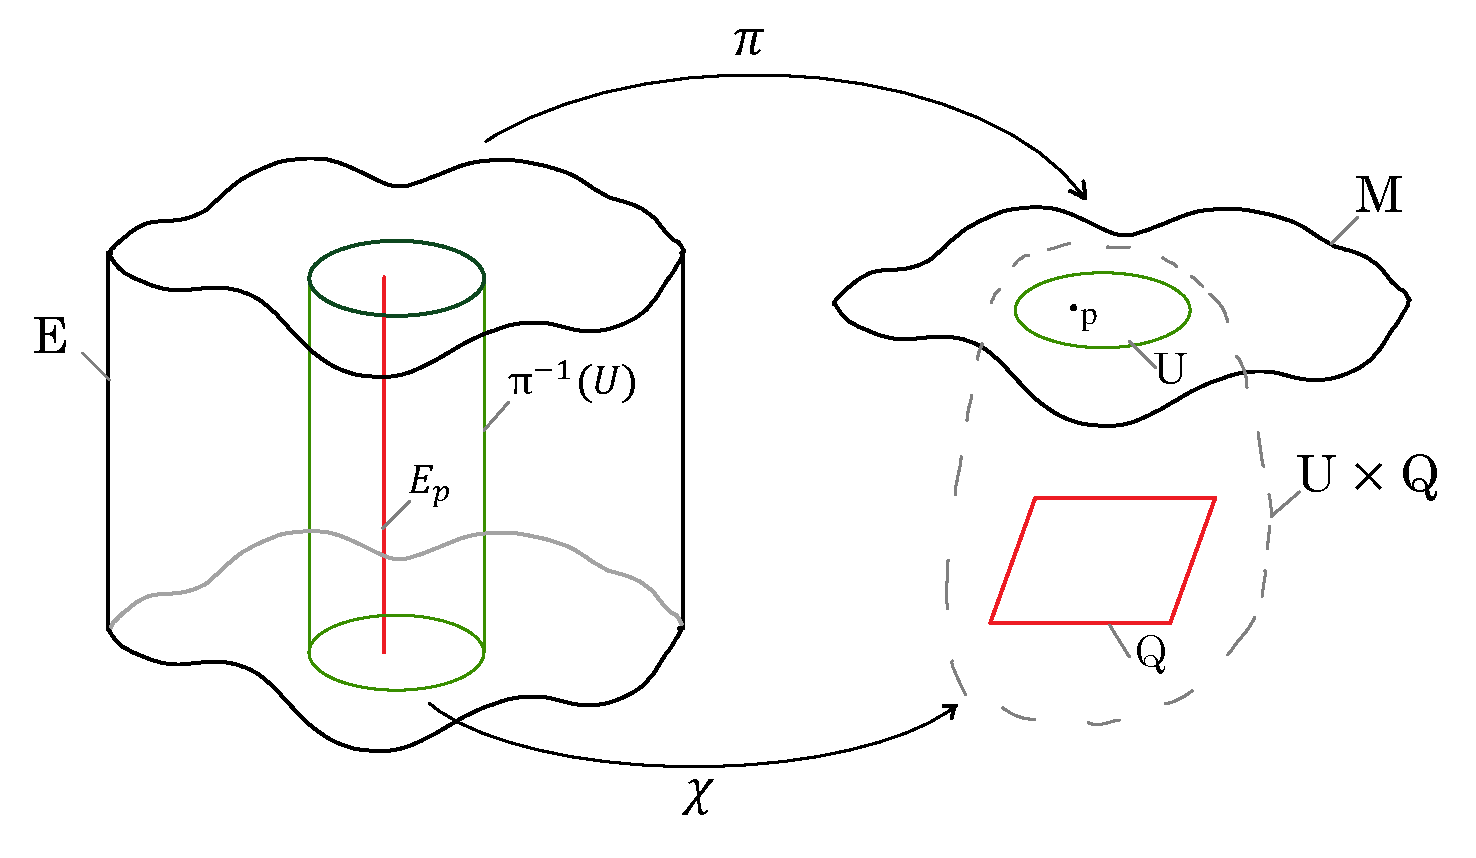
\includegraphics[width=0.8\textwidth]{../Pictures/fiberbundle}
  				\captionof{figure}{The complete fiber bundle Structure.}
			\end{figure}
			
			\begin{definition}[Smooth (cross) Section]
				We call \emph{Smooth (cross) Section} a smooth right-inverse function of $\pi$.\\
				I.e. any $\phi\in C^\infty(M;E)$ such that:
				\begin{compactdisplaymath}
					\pi\circ\phi = id|_M
				\end{compactdisplaymath}
			\end{definition}
			
			\begin{definition}[Bundle map (\emph{Fiber Preserving map})]\label{Def:BundleMap}
				We call \emph{bundle map} a smooth function $\phi: E \rightarrow E'$ such that:
			 	\begin{compactdisplaymath}
			 		\phi(E_{x})= F_{x} \qquad \forall x \in M.
			 	\end{compactdisplaymath}
				\textit{i.e.} the following graph commutes:

				\vspace{-2mm}
				\centering
				\begin{tikzpicture}
					 \matrix (m) [matrix of math nodes,row sep=3em,column sep=4em,minimum width=2em] {
						E & & F \\
       					& M & \\};
					\path[-stealth]
    					(m-1-1) edge node [left] {$\pi_{E}$} (m-2-2)
   		         		edge [right] node [above] {$\phi$} (m-1-3)
    					(m-1-3) edge node [right] {$\pi_{F}$} (m-2-2);
				\end{tikzpicture}
			\end{definition}
			
			\begin{definition}[Bundle of homomorphisms]
				We call \emph{bundle of homomorphisms} a fiber bundle $\Hom(E,E')$ over the base space $M$ such that the fiber over a base point $p\in M$ is the infinite dimensional manifold $\Hom(E_p,E'_p)$ isomorphic to $\Hom(Q,Q')$.
			\end{definition}

			\begin{definition}[Vector Bundle]
				We call \emph{Vector Bundle} a smooth bundle $E=(E,\pi,M;V)$ such that:
				\begin{compactitemize}
					\item The typical fiber $V$ is a finite dimensional vector space.
					\item All trivializations $\chi_{\alpha} $ are diffeomorphisms such that:
						\begin{compactdisplaymath}
							\left.\chi_{\alpha}\right\vert_{\pi^{-1}(p)} \in \mathbb{GL}(n, \mathbb{R})
							\quad : \; \pi^{-1}(p) \rightarrow \{p\}\times V \simeq V
						\end{compactdisplaymath}
				\end{compactitemize}
			\end{definition}

			\begin{definition}[Fibrewise inner product]
				We call \emph{inner product} of the vector bundle $E$ a smooth map:
				\begin{displaymath}
					<\cdot,\cdot> : E \times_M E \rightarrow \Real
				\end{displaymath}
				such that the restriction of $<\cdot,\cdot>$ to any fiber $E_p\times E_p$ is a non-degenerate bilinear form.
			\end{definition}
			
			\begin{definition}[Tangent Bundle]
				We call \emph{tangent bundle of M} the smooth vector bundle $TM=(TM,\tau,M;\Real^m)$ such that:
				\begin{compactitemize}
					\item The total space is the (disjoint) union of all tangent spaces to M :
						$$TM \coloneqq \underset{p \in M}{\sqcup} T_pM  \equiv \bigcup_{x\in M} {x}\times T_x M$$
					\item The bundle projection maps each tangent vector $v\in  T_pM$ to the correspondent base point  $p$;
						$$\tau : (p,v_p) \mapsto p $$
				\end{compactitemize}
			\end{definition}

				\begin{itemize}
				\item The \emph{Cotangent Bundle} $T^*M$ is  the vector bundle $T^*M$ builded by disjoint union of the dual tangent space $T_p^*M $.
					\item The \emph{Tensor Bundle} $T^{(k,l)}M$ is build by disjoint unions of the tensor product of tangent space with itself:
					\begin{displaymath}
						T^{(k,l)}_ p M = \underbrace{T^*_pM \otimes \cdots \otimes T^*_pM}_{\textrm{k-times}} \otimes
						\underbrace{T_pM \otimes \cdots \otimes T_pM}_{\textrm{l-times}}
					\end{displaymath}
					\item The \emph{k-form Bundle} $ \bigwedge^m( T^*M)$ is build by disjoint unions of the antisimmetrized tensor product of the dual tangent space with itself.
				\end{itemize}

				\begin{definition}[Tautological (Poincaré) 1-form]
						We call \emph{tautological form} the 1-form over $\Phase= T^*Q$:
						\begin{displaymath}
							\theta_0 \in \Gamma^\infty (T^*\Phase)
						\end{displaymath}
					such that the action on a generic point $ \omega_{\alpha_p} \in T_{\alpha_p}M$ ( in the fiber of $\alpha_p$, which in turn is a one-form on the fiber of $p\in Q$) is given by:
						\begin{displaymath}
						\theta_0 \big(\alpha_p \big): T_{\alpha_p}\Phase \rightarrow \Real \qquad : \; \omega_{\alpha_p} \mapsto \alpha_q \circ T \tau^*_Q \big( \omega_{\alpha_p} \big)
						\end{displaymath}
					where $T$ is the \emph{tangent map}, namely the bundle-morphism which act on each fiber as the differential map $d (\tau^*_Q)$.
					\end{definition}

					\begin{figure}[h!]
					  	\centering
   						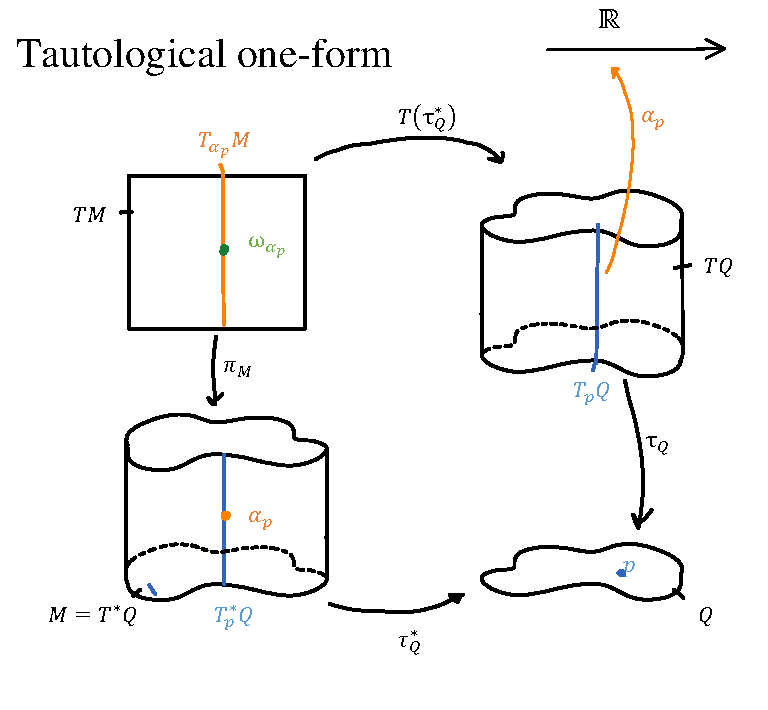
\includegraphics[width=0.7\textwidth]{../Pictures/Tautological1Form}
 						\caption{The definition of tautological 1-form is achieved exploiting the concept of \emph{Tangent map} and remembering that $\alpha_p: T_p \Phase \rightarrow \Phase$ is a linear functional.}
					\end{figure}

					\begin{definition}[Canonical (Poincarè)  symplectic form]\label{Def:NatSymForm}
						We call \emph{Canonical (Poincarè)} form the symplectic:
						\begin{displaymath}
							\omega_0 \coloneqq -d \theta_0
						\end{displaymath}
						In canonical coordinates it assumes the renown expression:
						\begin{displaymath}
							\omega_0 \coloneqq \sum_{i=1}^n  d q^i \wedge d p_i
						\end{displaymath}
					\end{definition}
					
					
		\subsection{Jet Bundles}\label{Sect:JetBundles}
			The jet bundle is a %certain
			construction that makes a new smooth fiber bundle out of a given bundle. 
			
			\begin{definition}[r-jet equivalence]
				Two sections $\sigma, \eta \in \Gamma^\infty(p)$ have the \underline{same \emph{r-jet} at $p$} $(\sigma \sim \eta)$ iff:
				\begin{displaymath}
					\left.\frac{\partial^{|I|} \sigma^{\alpha}}{\partial x^{I}}\right|_{p} = \left.\frac{\partial^{|I|} \eta^{\alpha}}{\partial x^{I}}\right|_{p} \quad \forall I\in \Natural^m_0 \, \vert \, 0 \leq |I| \leq r.
				\end{displaymath}
				where $I$ is a \emph{multi-index} ,see Remark \ref{MultiIndex}.
		\end{definition}
		\begin{remark}\label{MultiIndex}
			(multi-index notation)
			\\
			A multi-index is a %natural valued
			finite dimensional vector  $I=(i_1, i_2, \ldots, i_m)\: \in \Natural^m_0$ with $m<\infty$.
			\\
			On $\Real^n$ a differential operator can be identified by a multi-index:
			\begin{displaymath}
				\frac{\partial^{|I|}}{\partial x^{I}} := \prod_{i=1}^{m} \left( \frac{\partial}{\partial x^{i}} \right)^{I(i)}
			\end{displaymath}
			(Whenever the Schwartz theorem holds, the order of derivation is irrelevant.)
			\\
			The order of the multi-index is defined as:
			\begin{displaymath}
				|I| := \sum_{i=1}^{m} I(i)
			\end{displaymath}
		\end{remark}

		\begin{definition}[Space of r-th Jet in p]
			We call \emph{space of the r-th jet in p} the set of the equivalence class under the jet equivalence relation.
			\begin{displaymath}
				J^r_{\,p}(E) \coloneqq \frac{\Gamma^\infty(p)}{\sim}
			\end{displaymath}
			where $\sim$ is the r-Jet equivalence.
		\end{definition}
		\begin{notationfix}
			A r-jet with representative $\sigma$ is denoted as $j^r_p\sigma$ .
			\\
			The integer $r$ is also called the order of the jet, $p$ is its source and $\sigma(p)$ is its target.
		\end{notationfix}

		\begin{definition}[r-th Jet Bundle of $E$]
			We call \emph{r-th Jet Bundle of $E$} the smooth bundle $(J^r(E), \pi_r, M)$	where:
			\begin{compactitemize}
				\item $J^r(E) \coloneqq \underset{p \in M}{\sqcup} J^r_p (E)
					 \equiv \big\{j^r_p\sigma \quad \vert \; p\in M, \; \sigma \in \Gamma^\infty(p) \big\}$
				\item $\pi_r: J^r(E) \rightarrow M$ such that $j^{r}_{p}\sigma \mapsto p $
			\end{compactitemize}
		\end{definition}					
					

			\begin{definition}[(Pseudo-Riemannian) Metric]
				We call \emph{(Pseudo-Riemannian) Metric} a map on the bundle product of $TM$ with itself:
				$$g: TM \times_M TM \rightarrow \Real$$
				such that the restriction on each fiber $$g_p: T_pM \times T_pM \rightarrow \Real $$ is a non-degenerate bilinear form.
			\end{definition}

			\begin{definition}[Pseudo-Riemannian Manifold]
				We call \emph{Pseudo-Riemannian manifold} a pair $(M, g)$ such that:
				\begin{compactitemize}
					\item $M$ is a n-dimensional $(n\geq2)$, Hausdorff, second countable, connected, orientable smooth manifold.
					\item $g$ is a Pseudo-Riemannian metric.
				\end{compactitemize}
			\end{definition}					
	
			\begin{definition}[Time-orientation]
				We call \emph{time-orientation} a global tangent vector field  $\mathfrak{t}\in \Gamma^\infty(TM)$ over the Lorenzian manifold $M$
				such that:
				\begin{compactitemize}
					\item $\supp(\mathfrak{t}) = M$
					\item $\mathfrak{t}(p)$ is time-like $\forall p \in M$.
				\end{compactitemize}
			\end{definition}

			\begin{definition}[Spacetime]
				We call \emph{spacetime} a quadruple $(M, g, \mathfrak{o}, \mathfrak{t})$ such that:
				\begin{compactitemize}
					\item $(M,g)$ is a time-orientable\footnote{Manifold for which such \emph{time-orientation} exists.} n-dimensional Lorentzian manifold $(n>2)$
					\item $\mathfrak{o}$ is a choice of orientation
					\item $\mathfrak{t}$ is a choice of time-orientation
				\end{compactitemize}
			\end{definition}				

			\begin{definition}[Achronal Set]
				We call \emph{achronal set} a subset $\Sigma \subset M$ such that every inextensible timelike curve intersects $\Sigma$ at most once.
			\end{definition}

			\begin{definition}[$\substack{\textrm{ future}\\ \textrm{past } } $ Domain of dependence of an Achronal set]
				We call \emph{$\substack{\textrm{ future}\\ \textrm{past } } $ domain of dependence} of an achronal set  $\Sigma \subset M$, the two subset:
				\begin{displaymath}
					\mathbf{D}_M^\pm(\Sigma) \coloneqq \big\{ q \in M \big\vert \; \forall \gamma \substack{\textrm{ past}\\ \textrm{ future} }\textrm{\footnotesize inextensible causal curve passing through }q : \; \gamma(I) \cap \Sigma \neq \emptyset  \big\}
				\end{displaymath}
			\end{definition}
			
			\begin{definition}[Cauchy Surface]
				We call \emph{Cauchy surface} a closed, achronal subset $\Sigma \subset M$ such that:
				\begin{displaymath}
					\mathbf{D}_M(\Sigma) \equiv M
				\end{displaymath}
			\end{definition}
			
			\begin{notationfix}
				We denote the set of all the Cauchy surfaces as $\gls{CauchyClass}$.
			\end{notationfix}
			
		\begin{definition}[Globally-Hyperbolic SpaceTime]\label{Def:GHSP}
			We call a spacetime $M$ \emph{globally hyperbolic} if it contains at least one \emph{Cauchy Surface}.
		\end{definition}					

			\begin{notationfix}
				Let $M$ be a globally hyperbolic spacetime and $E=(E,\pi,M;V)$ a vector bundle of typical fiber $V$.\\
				We denote:
				\begin{itemize}
							\renewcommand\labelitemi{$\cdot$}
					\item $\Gamma_0(E)$ the space of \emph{compactly supported} smooth sections.
					\item $\Gamma_{sc}(E)$  the space of \emph{spacelike compact} smooth sections.\\
						$\big(\; f\in \Gamma_{sc}(E)$ if there exists a compact subset $K \subset M$  such that $\supp f \subset \mathbf{J}_M(K)$. $\big)$
					\item  $\Gamma_{fc}(E) $ the space of \emph{future- compact} smooth sections.\\
						$\big(\; f\in \Gamma_{fc}(E) $ if  $\supp(f) \cap  \mathbf{J}^+_M(K)$ is compact for all $p\in M$.$\big)$
					\item  $\Gamma_{pc}(E) $ the space of \emph{past- compact} smooth sections.\\
						$\big(\; f\in \Gamma_{pc}(E) $ if  $\supp(f) \cap  \mathbf{J}^-_M(K)$ is compact for all $p\in M$.$\big)$
					\item $\Gamma_{tc}(E) \coloneqq \Gamma_{pc}(E) \cap \Gamma_{fc}(E) $ the space of \emph{timelike compact} smooth sections.
				\end{itemize}
			\end{notationfix}

		\begin{definition}[Linear Partial Differential operator \footnotesize( of order at most $s\in \Natural_0$)]\label{Def:LPDO}
			We call \emph{linear partial differential operator} a
			linear map $L:\Gamma(E)\rightarrow \Gamma(E')$ such that $\forall p \in M$ there exists:
		\begin{itemize}
			%\item open set $U \ni p$.
			%\item $(U, \varphi )$ local chart on $M$.
			%\item $(U, \chi)$ local trivialization of $F$
			%\item $(U, \chi')$ local trivialization of $F'$
			\item $U \ni p$ open set rigged with:
				\begin{itemize}
					\item $(U, \varphi )$ local chart on $M$.
					\item $(U, \chi)$ local trivialization of $F$
					\item $(U, \chi')$ local trivialization of $F'$
				\end{itemize}
			\item $\{A_\alpha :U \rightarrow \Hom(V,V')\; \vert \: \alpha \in \Natural_0^n, \vert \alpha \vert \leq s \}$
			a collection of smooth maps labeled by multi-indices where $s$ is a fixed integer said \emph{order of the operator}.
		\end{itemize}
		which allows to express $L$ locally:
		\begin{displaymath}
			\chi' \circ ( L \sigma) \circ \varphi^{-1} =
			\sum_{\vert \alpha \vert \leq s} A_\alpha \partial^\alpha (\chi \circ \sigma \circ \varphi^{-1} )
			\qquad \forall \sigma \in \dom(L) \subset \Gamma(E)
		\end{displaymath}
		(where we have make use of the multi-index notation\ref{MultiIndex})
	\end{definition}
				\begin{definition}[Formal Dual Operator ( of $L$)]
				We call \emph{formal dual operator} of $L$
				the unique linear partial differential operator $L^\star: \Gamma(G^*) \rightarrow \Gamma(E^*)$ such that:
				\begin{displaymath}
					<L^\star g' , f > = <g', L f>
				\end{displaymath}
				$\forall f\in \Gamma(E),\; g' \in \Gamma(G^*)$ which have supports with compact overlap.
				\\
				($<\cdot,\cdot>$ denotes the 1-form evaluation: $<\alpha,v>= \alpha(v) \quad \forall v\in E_p, \alpha \in E^*_p$.)
			\end{definition}

			\begin{definition}[$\substack{\textrm{ retarded}\\ \textrm{advanced } } (\pm)$ Green Operators]\label{Def:GreenOperators}
				We call \emph{$\substack{\textrm{ retarded}\\ \textrm{advanced } } (\pm)$ Green Operator} of $L$ a
				l.p.d.o. $G^\pm : \Gamma (E) \rightarrow \Gamma(E)$ such that:
				\begin{compactitemize}
					\item $\dom(G^+) = \Gamma_{pc}(E) \qquad \dom(G^-) = \Gamma_{fc}(E)$
					\item $LG^\pm f=G^\pm Lf = f \qquad \forall f\in \dom(G^\pm)$
					\item $\supp(G^\pm f) \subset \mathbf{J}^\pm_M (\supp(f)) \qquad \forall f\in \dom(G^\pm)$
				\end{compactitemize}
				In others words we can say that
				$G^\pm$ is the left-right inverse of the restriction of $L$ to $\dom(G^\pm)$.
			\end{definition}

			\begin{notationfix}

				We call \emph{Advanced minus Retarded operator} or \emph{Causal Propagator}\cite{Benini2013} the operator:
				\begin{displaymath}
					E \coloneqq G^-  - G^+ : \Gamma_{tc}(E) \rightarrow \Gamma(E)
				\end{displaymath}
			\end{notationfix}

			\begin{definition}[Green hyperbolic operator]
				We call \emph{Green hyperbolic} a
%				The
				linear partial differential operator $P$
%				is be called Green hyperbolic if
				such that $P$ and $P^\star$ have advanced and retarded Green’s operators.
			\end{definition}
			For these operators uniqueness of Green's operators is guaranteed:
			\begin{theorem}[Characterization of Green Hyperbolic operators]\label{Teo:GreenHypCharacter}
				$ $
				\begin{hypothesis}
					\begin{itemize}
						\item $E=(E,\pi,M)$ a vector bundle over a globally hyperbolic spacetime $M$.
						\item $P:\Gamma(E) \rightarrow \Gamma(E)$ a Green hyperbolic operator, $G^\pm$ its Green's operators and $G_\star^\pm$ the Green's operators of the dual.
					\end{itemize}
				\end{hypothesis}
				\begin{thesis}
					\begin{itemize}
					\item $P$ possesses a unique retarded $\GreenRet$ and a unique advanced $\GreenAdv$ Green's operator.
					\item $<G_\star^\pm f', f> = <f', G^\mp f > \qquad \forall f \in \Gamma_0(E),\: \forall f' \in \Gamma_0(E^*)$
					\end{itemize}
				\end{thesis}
			\end{theorem}
	
\begin{definition}
A Poisson algebra is a Triple $\left(V, \cdot ,\{ , \} \right)$ space]]  where:
\begin{itemize}
	\item $V$ is a vector space of field $K$
	\item $ \cdot : V \times V \rightarrow \Real$  and $\{ , \} : V \times V \rightarrow \Real$ are bilinear products
\end{itemize}
such that:
\begin{itemize}
\item The product $ \cdot $ forms an  associative $K-$algebra.
\item The product $\{ , \}$, called the \emph{Poisson Brackets}  is anti-symmetric, obeys the\emph{Jacobi Identity} (i.e. forms a Lie Algebra)
\item The Poisson bracket acts as a derivation of the associative product $ \cdot $, i.e. for any three elements $x,y,z$ in the algebra, one has
\begin{displaymath}
	\{x, y \cdot z \} = { x , y } \cdot z + y \cdot { x , z }
\end{displaymath}
\end{itemize}
\end{definition}
				
\end{document} %\/\/\/\/\/\/\/\/\/\/\/\/\/\/\/\/\/\/\/\/\/\/\/\/\/\/\/\/\/\/\/\/\/\/\/\/\/\/\/\/\/\/\/\/\/\/\/\/\/\/\/\/\/\/\/\/\/\/\/\
%\/\/\/\/\/\/\/\/\/\/\/\/\/\/\/\/\/\/\/\/\/\/\/\/\/\/\/\/\/\/\/\/\/\/\/\/\/\/\/\/\/\/\/\/\/\/\/\/\/\/\/\/\/\/\/\/\/\/\/\/\/\/\/\/\/\/\/\/\/
